\begin{otherlanguage}{ngerman}
\section{Methodik}
\subsection{Virtuelle Umgebung}\label{Praktisches Terraform}
Um eine sichere virtuelle Umgebung zu schaffen, werden zwei Server benötigt. Ein Server bearbeitet DNS-Anfragen und der andere Server ist mit Malwareanalyse-Tools ausgestattet. Zudem sind keine Verbindungen zugelassen, außer Port 22. Dieser ist der SSH-Port und bietet hier die Möglichkeit den Server von außen zu beobachten. Ansonsten besteht die Möglichkeit für den Analyseserver sich mit dem Server zu verbinden der ein Netzwerk simuliert. Das ist daher nötig, da Malware teilweise nur mit Internetverbindung funktioniert. 
\subsubsection{Konfiguration der Umgebung}
Wie bereits beschrieben besteht die Cloud-Umgebung aus zwei Servern und einem Rechner, der Zugriff auf die Server hat.
\begin{figure}[h!]
    \centering
    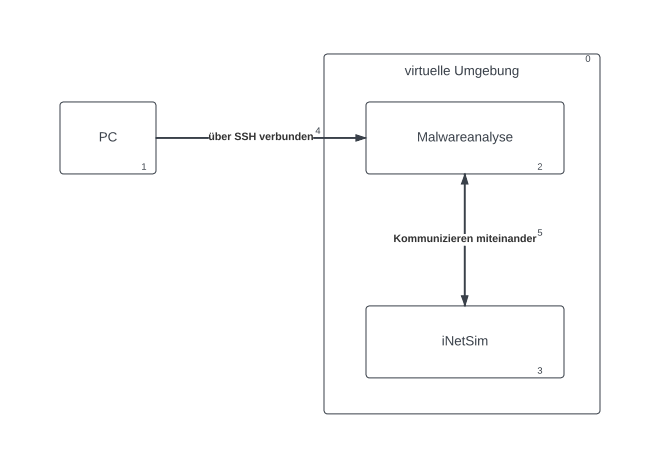
\includegraphics[scale=0.7]{LaTeX/graphic/virtuelleUmgebung.png}
    \caption{Aufbau der Cloud-Umgebung}
\end{figure}
\newline
In Abbildung zwei ist dieser Aufbau bildlich dargestellt. Auf der rechten Seite befindet sich die virtuelle Umgebung (mit null gekennzeichnet). Auf ihr laufen die beiden virtuellen Server. Einer der Server ist für die Malware-Analyse zuständig (mit zwei gekennzeichnet). Hier sind die Tools vorzufinden und die Malware wird hier eingeschleust. Außerdem gibt es den zweiten virtuellen Server, welcher ein Netzwerk simuliert (mit drei gekennzeichnet). Dafür wird das Programm \dq iNetSim \dq{} verwendet. Dieses simuliert gängige Internetdienste und ist dafür gemacht bei der Malware-Analyse eingesetzt zu werden.
\newline
Diese beiden Server können über jeden Port miteinander kommunizieren, haben aber keine Verbindung nach außen, sondern bleiben in der geschlossenen Umgebung. Die Kommunikation der beiden Server ist in der Abbildung mit fünf gekennzeichnet. Die einzige weitere Verbindung die in diesem System hergestellt wird ist die Verbindung vom PC des Benutzers auf den Malware-Analyseserver über SSH (mit vier gekennzeichnet). Somit wird gewährleistet, dass man als Analyst der Malware das System steuern und beobachten kann. 
\newline
Anhand des Aufbaus der Umgebung ist auch zu erkennen wie abgekapselt das System ist. Es bestehen keine Verbindungen nach außen, sondern nur untereinander, bzw von außen nach innen. Das ist auch wichtig um das Ausdringen der Malware zu verhindern. Diese Regeln für die Kommunikation sind in den Firewallregeln festgehalten. 
\subsection{Terraform}
\subsubsection{Verbindung mit dem Cloud-Provider}
Um Terraform als Provisioning-Tool für Cloud-Umgebungen zu verwenden, muss eine Verbindung zwischen der Terraform-Umgebung und dem Provider vorhanden sein. Diese Verbindung wird über ein API-Token geschaffen. Ein API-Token ist
\subsubsection{Konfiguration der Server}
In Terraform können Server erstellt und entsprechend konfiguriert werden. Wie das gemacht wird, wird hier einmal aufgegriffen. 
\newline
In HCL werden Blocks für die Erstellung von vielen Komponenten verwendet, darunter auch für die Servererstellung. 
\tt  
\begin{lstlisting}[caption = Konfiguration Malware-Server, language=python, numbers=left, numberstyle=\tiny]
# Create a server
resource "hcloud_server" "malware" {
  name        = "malware"
  image       = "ubuntu-22.04"
  server_type = "cx11"
  firewall_ids = [hcloud_firewall.saferfw.id]
  ssh_keys = [hcloud_ssh_key.default.id]
  user_data = file("user_data.yml")

public_net {
    ipv4_enabled = true
    ipv4 = hcloud_primary_ip.primary_ip_Malware.id
    ipv6_enabled = false
  }
}
\end{lstlisting}
\rm
Der abgebildete Code ist die Konfiguration für einen Server in der \dq Hetzner-Cloud\dq. Das ist bereits in Zeile zwei hinter \dq resource \dq{} zu erkennen. Der hier erstellte Server trägt den Namen \dq malware \dq{} und hat als Betriebssystem \it Ubuntu \rm (Vgl. Zeile vier). Der Server-Typ (Zeile 5) legt fest, welche Cloud-Lösung des Providers verwendet werden soll. In der \dq Hetzner-Cloud \dq{} ist \dq cx11\dq{} die günstigste Version. Diese ist für die grundlegende Malware-Analyse dennoch ausreichend. Falls die Analyse durch stärkere Systemkomponenten beschleunigt werden soll, kann hier der Typ geändert werden. 
\newline
Im Anschluss daran wird dem Server eine Firewall zugewiesen. Welche Einstellungen diese hat wird im nächsten Unterpunkt genauer betrachtet. Daraufhin bekommt der Server die Info woher der SSH-Key genommen wird (Zeile sieben). In Zeile zehn werden die öffentlichen Netzwerkeinstellungen vorgenommen. Dazu wird festgelegt, welche \dq Internet-Protokoll-Version \dq{} vorhanden ist. In diesem Fall ist \dq IPv4 \dq{} erlaubt und \dq IPv6 \dq{} nicht. Die \dq IPv4 \dq-Adresse wird dem Server fest zugewiesen. Das ist für die spätere Kommunikation mit dem anderen Server wichtig.
\newline
\newline
\tt  
\begin{lstlisting}[caption = Konfiguration iNetSim-Server, language=python, numbers=left, numberstyle=\tiny]
#Create second Server
resource "hcloud_server" "iNetSim" {
  name        = "iNetSim"
  image       = "ubuntu-22.04"
  server_type = "cx11"
  firewall_ids = [hcloud_firewall.iNetSimFW.id]
  ssh_keys = [hcloud_ssh_key.default.id]
  
  public_net {
    ipv4_enabled = true
    ipv4 = hcloud_primary_ip.primary_ip_iNetSim.id
    ipv6_enabled = false
  }
}
\end{lstlisting}
\rm
Die Konfiguration des zweiten Servers ist, wie hier zu sehen, sehr ähnlich zu der des ersten Servers. Der Unterschied hier ist nur die zugewiesene Firewall (Zeile sechs) und die IP-Adresse (Zeile elf). 
\subsubsection{Konfiguration der Firewall}
Die Erstellung einer sicheren und durchdachten Firewall ist bei der Arbeit mit Malware sehr wichtig, um Schäden am eigenen oder fremden Systemen zu vermeiden. 
\newline
\newline
\tt
\begin{lstlisting}[caption = Konfiguration der Firewall für den Analyseserver, language=python, numbers=left, numberstyle=\tiny]
#Create a firwall
resource "hcloud_firewall" "saferfw" {
  name = "saferfw"
  rule {
    direction = "in"
    protocol  = "tcp"
    port      = "22"
    source_ips = [
      "0.0.0.0/0",
      "::/0"
    ]
  }

  rule {
    direction = "out"
    protocol  = "udp"
    port = "1-65535"
    source_ips = [
      hcloud_primaryip.primary_ip_iNetSim.id
    ]
  }

  rule {
    direction = "out"
    protocol = "tcp"
    port = "1-65535"
    source_ips = [
      hcloud_primaryip.primary_ip_iNetSim.id
    ]
  }
}
\end{lstlisting}
\rm
Dieser Code stellt die Definition der Firewall für den Malware-Analyseserver dar. Der Name dieser Firewall ist \dq saferfw \dq{} und sie besteht aus drei Regeln. Die erste Regel (Zeile vier bis elf) legt die Kommunikation über den SSH-Port fest. Diese ist nur nach innen zugelassen. Wer diese Verbindung zum Server herstellt ist egal, solange der SSH-Key stimmt. 
\newline

\end{otherlanguage}